\part{Data-driven decision making}
\frame{\partpage}

\begin{frame}
	\begin{center}
		
\includegraphics[width=0.6\textwidth]{valve_logo}
		
		\url{https://youtu.be/HQwL6zh7AgA}
		
		\url{http://media.steampowered.com/apps/steamdevdays/slides/data.pdf}
	\end{center}
\end{frame}

\begin{frame}{Decision making at Valve}
	\begin{itemize}
		\pause\item Valve favour \textbf{data-driven decision making}
			\begin{itemize}
				\pause\item Ask \textbf{explicit} questions
				\pause\item Look at the \textbf{data}
				\pause\item Use the data to develop a \textbf{theory}
				\pause\item Define \textbf{measurable outcomes}
				\pause\item \textbf{Iterate}
			\end{itemize}
	\end{itemize}
\end{frame}

\begin{frame}
	\begin{tikzpicture}[remember picture, overlay]
		\node[at=(current page.center)] {
			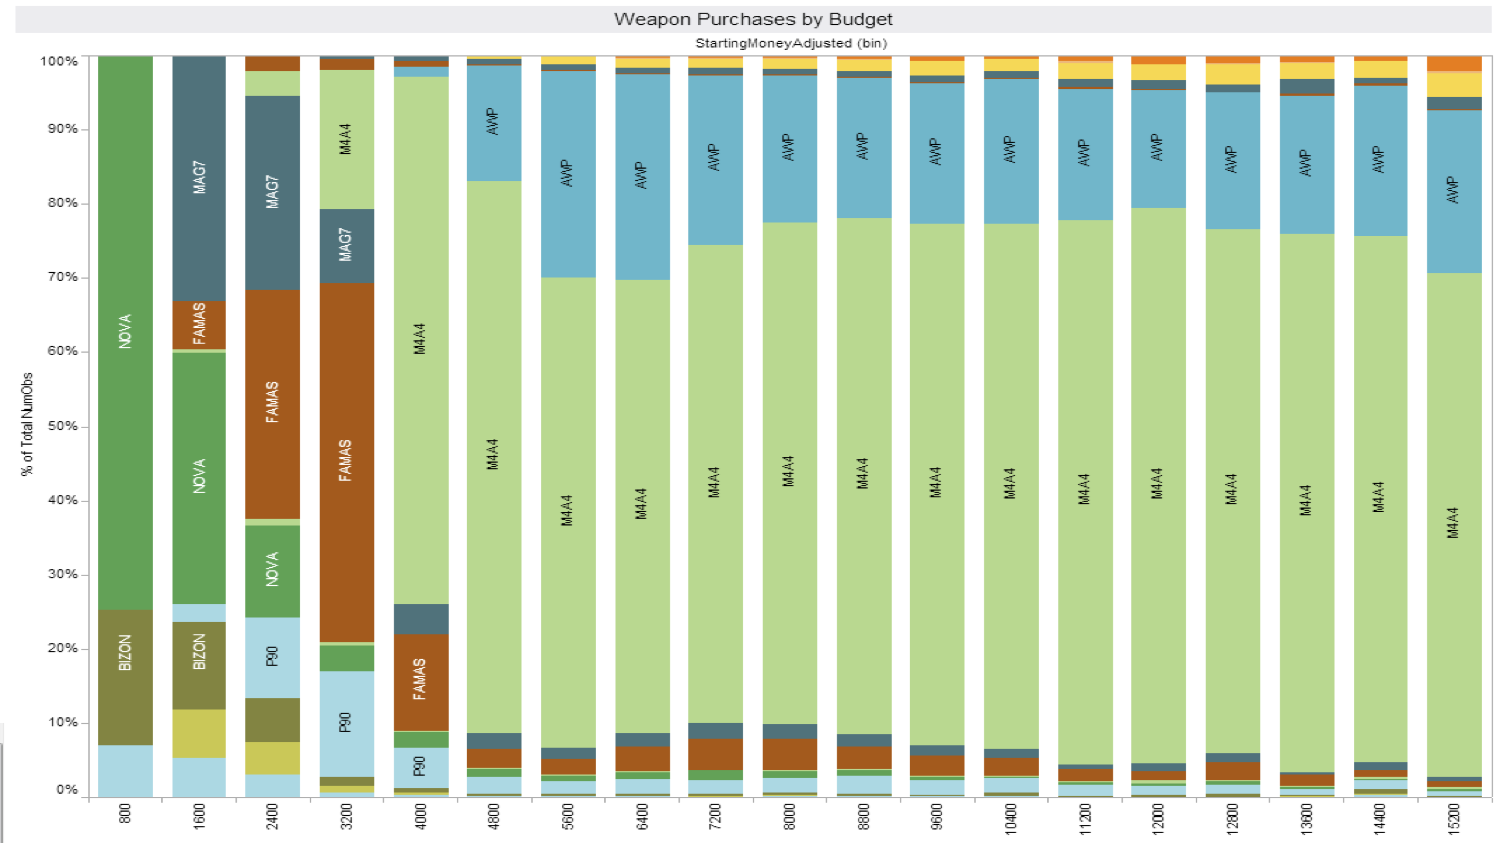
\includegraphics[width=\paperwidth]{csgo_1}
		};
	\end{tikzpicture}
\end{frame}

\begin{frame}
	\begin{tikzpicture}[remember picture, overlay]
		\node[at=(current page.center)] {
			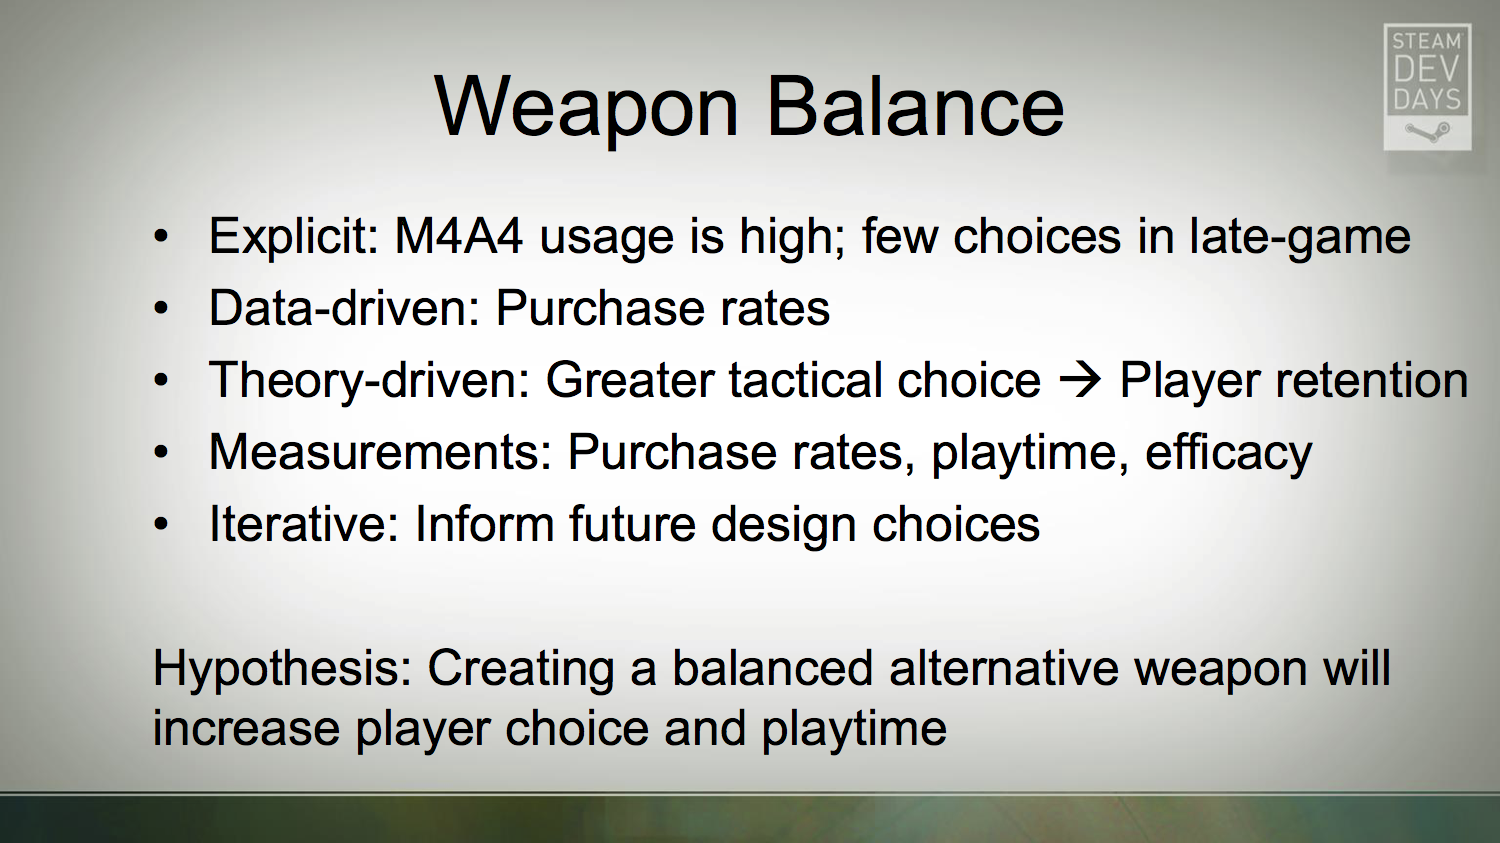
\includegraphics[width=\paperwidth]{csgo_2}
		};
	\end{tikzpicture}
\end{frame}

\begin{frame}
	\begin{tikzpicture}[remember picture, overlay]
		\node[at=(current page.center)] {
			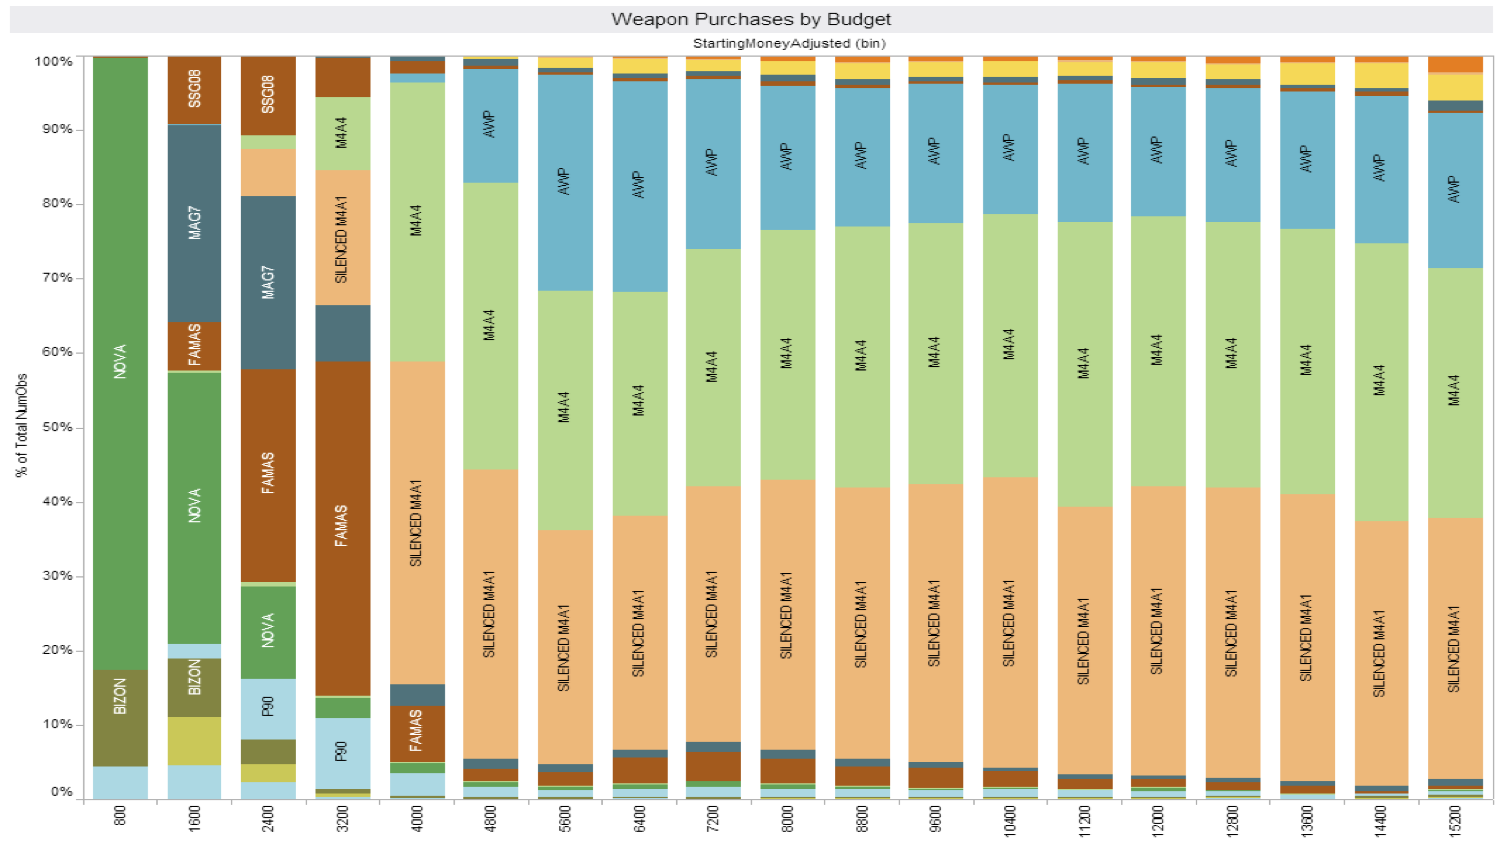
\includegraphics[width=\paperwidth]{csgo_3}
		};
	\end{tikzpicture}
\end{frame}

\begin{frame}
	\begin{tikzpicture}[remember picture, overlay]
		\node[at=(current page.center)] {
			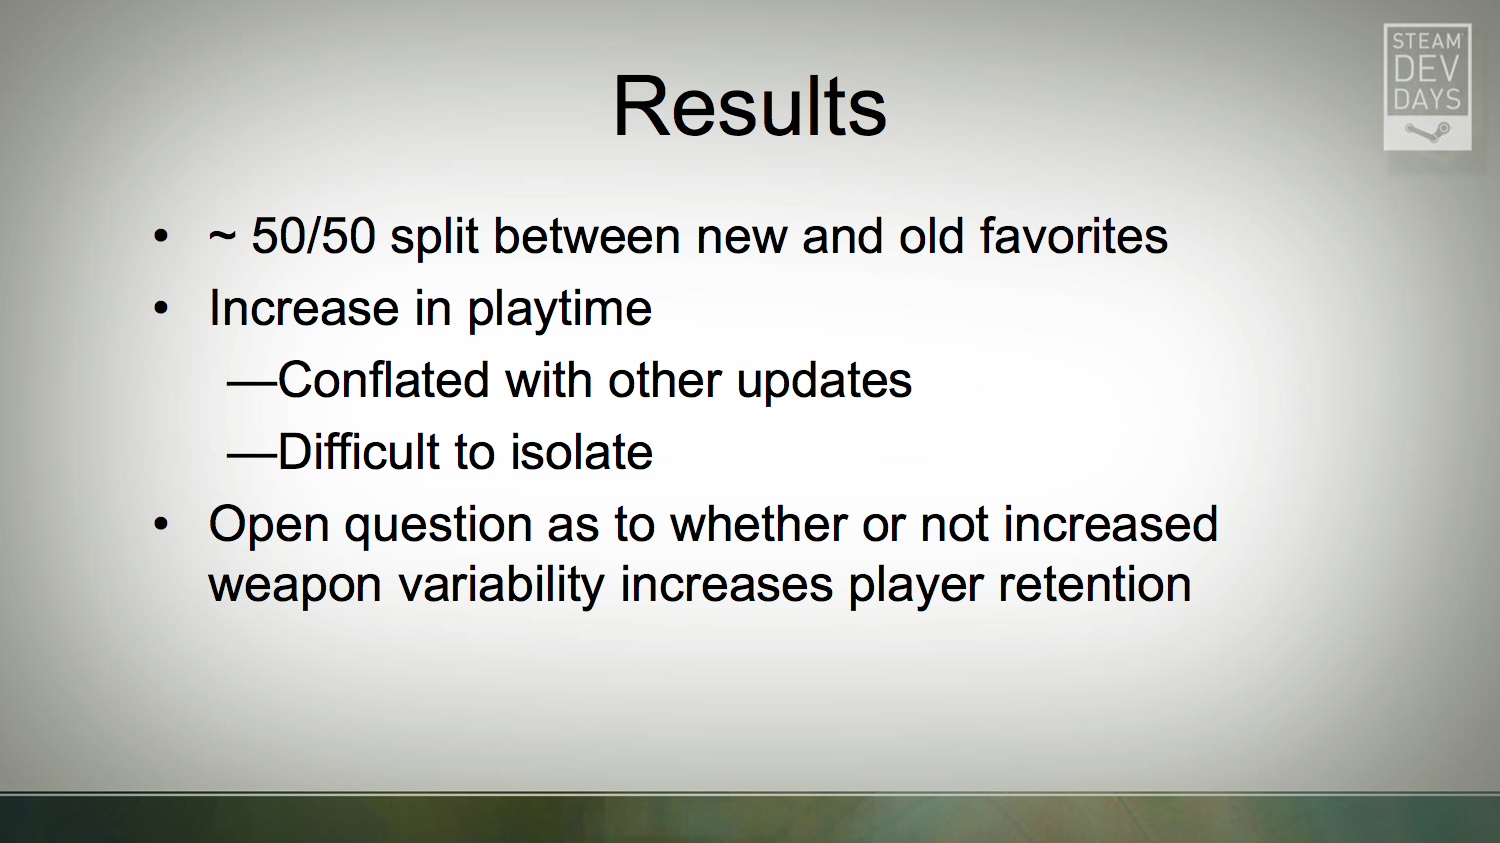
\includegraphics[width=\paperwidth]{csgo_4}
		};
	\end{tikzpicture}
\end{frame}

\begin{frame}{Data visualisation}
	\begin{tikzpicture}[remember picture, overlay]
		\node[at=(current page.south), anchor=south] {
			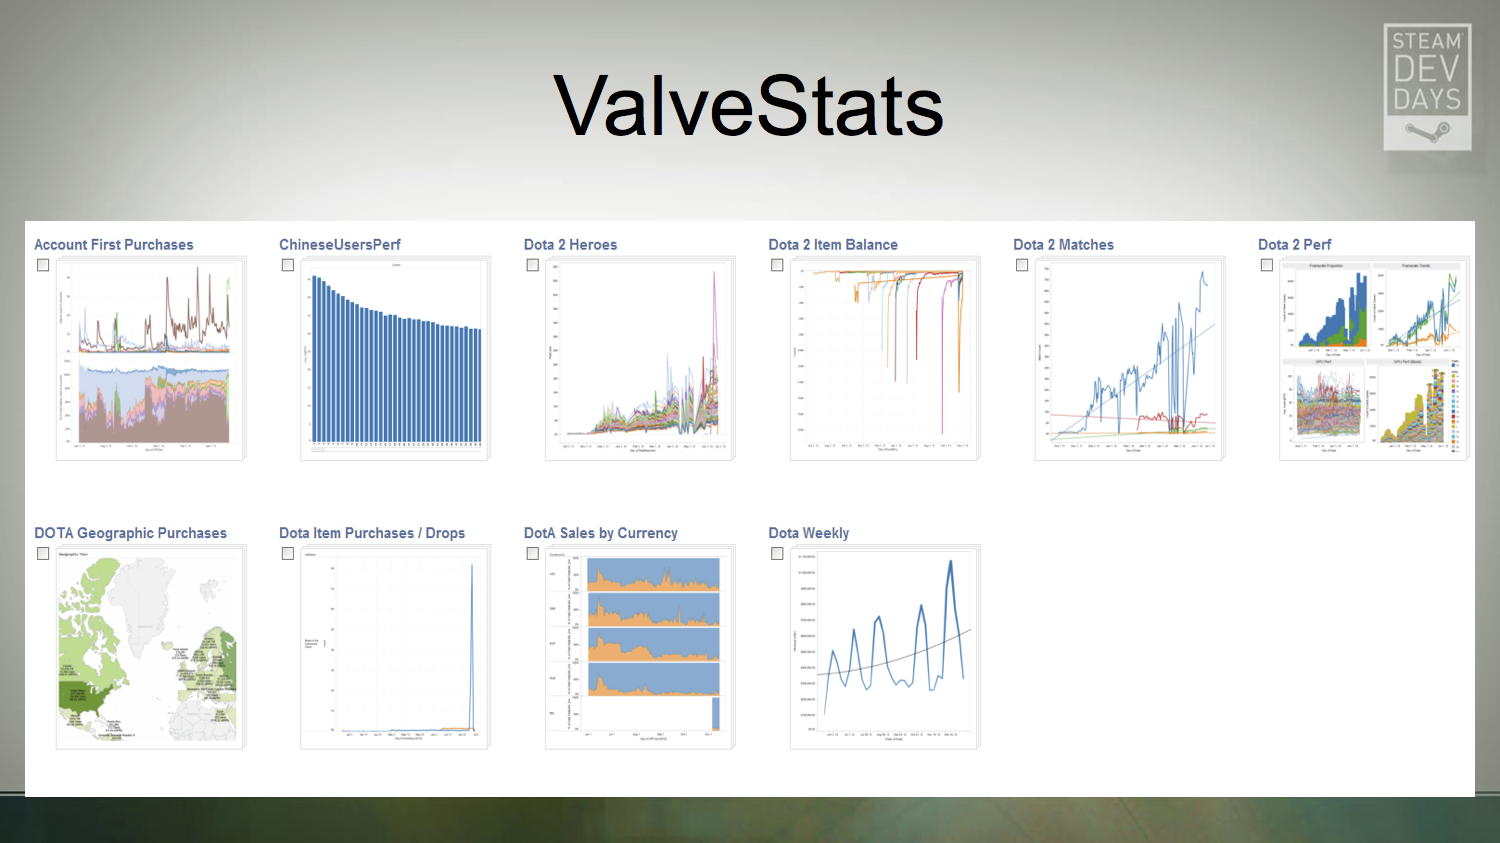
\includegraphics[width=\paperwidth]{valve_stats}
		};
	\end{tikzpicture}
\end{frame}

\begin{frame}{Player deaths in Team Fortress 2}
	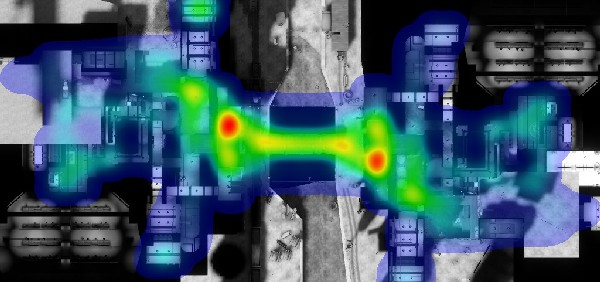
\includegraphics[width=\textwidth]{heatmap_tf2}
\end{frame}

\begin{frame}{Weapon fire locations in CS:GO}
	\begin{center}
		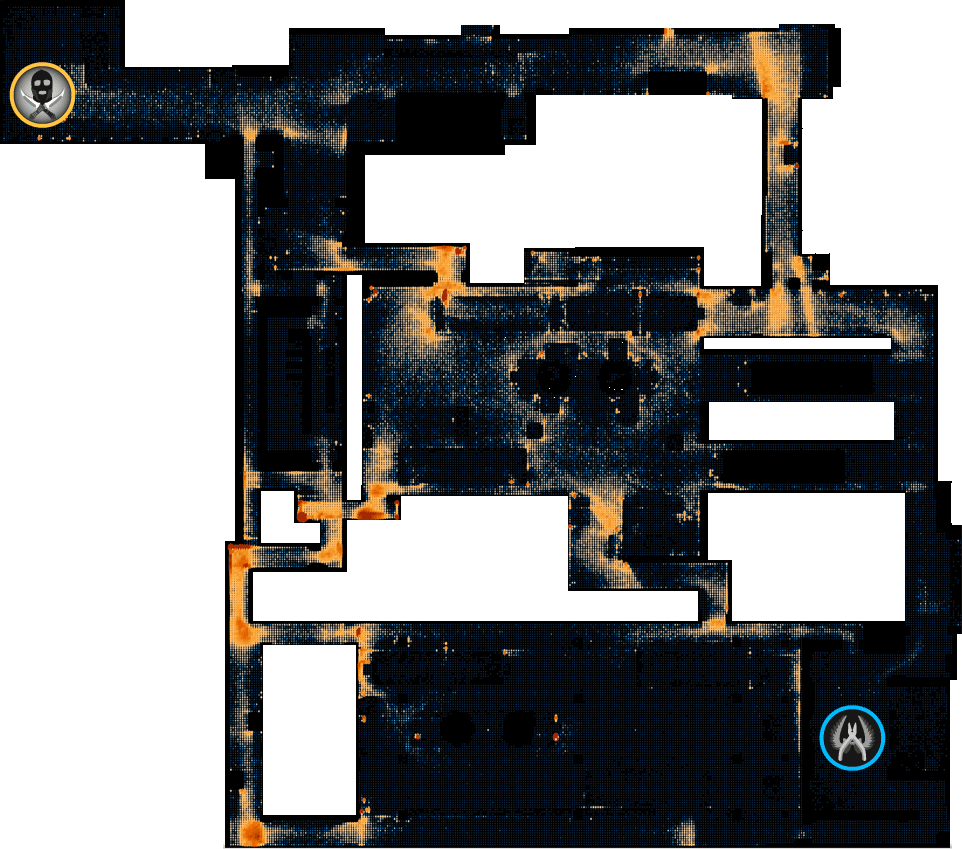
\includegraphics[height=0.8\textheight]{heatmap_csgo}
	\end{center}
\end{frame}

\begin{frame}{Data visualisation}
	\begin{itemize}
		\pause\item Humans are good at seeing \textbf{patterns}
		\pause\item Good data visualisation can help to spot patterns
		\pause\item ... However this should be followed up by proper statistical analysis!
	\end{itemize}
\end{frame}
